\section{Sec.~IV: Von Neumann algebras and entanglement: type III}

This is the technical heart of the whole paper, and it earns that description honestly: type III algebras have
no trace, so eqs.~3.1--3.2 (the density operator $\rho_\M$ and the entropy $S_\M$) simply cannot be written
down — there is no equation left to solve. And yet, as flagged repeatedly, type III is not some exotic
mathematical curiosity to be handled as a special case; it is the type that governs local regions of a
relativistic quantum field theory, and (as Sec.~VII will show) the type that governs holographic boundary
algebras in the strict large-$N$ limit. If the goal is to say anything at all about entanglement in exactly
the settings this paper cares about most, an entirely different tool is needed. That tool is
\textbf{Tomita--Takesaki modular theory}, and the core physical idea behind it is worth stating in one sentence
before any formalism: \emph{when a subsystem is highly entangled with its complement, not knowing about the
complement makes the subsystem look thermal} — entanglement, viewed from inside just one half, always looks
like heat. Everything in this section is that one idea, made completely precise.

\subsection{Sec.~IV.A: emergent times from entanglement — modular flows}

\subsubsection*{Starting from something you already understand: the type I case, retold}

To motivate the general construction, go back to an ordinary type I bipartite pure state $\ket\Psi$ with
full-rank reduced density matrix $\rho_R$ (``full-rank'' meaning invertible — every eigenvalue strictly
positive, so $\rho_R^{-1}$ exists; this will matter in a moment). Instead of studying the entropy $S_R$
directly, package the same information differently: write
\[
\rho_R = e^{-K_R}, \qquad K_R\equiv-\log\rho_R
\]
(eq.~4.1). $K_R$ is called the \textbf{entanglement Hamiltonian}, and $K_R\ge0$ (since $\rho_R$'s eigenvalues
are all in $(0,1]$, their negative logarithms are all $\ge0$). The full set of eigenvalues of $K_R$ — the
\emph{entanglement spectrum} — carries strictly more information than the entropy $S_R$ alone or any finite
list of R\'enyi entropies (each of those is just some specific weighted sum over the spectrum; the full
spectrum is the un-summed data), which is why condensed-matter physicists studying entanglement spectra
directly (rather than just the single number $S_R$) have found it such a fruitful diagnostic tool.

Now use $K_R$ to generate a flow:
\[
A(s) = e^{iK_Rs}Ae^{-iK_Rs} \in B(\HH_R), \qquad A\in B(\HH_R)
\]
(eq.~4.2) — this is formally identical to ordinary Heisenberg time evolution, $A(t)=e^{iHt}Ae^{-iHt}$, with
$K_R$ playing the role of a Hamiltonian and $s$ playing the role of time. It's called \textbf{modular flow},
and $s$ is called \textbf{modular time}. The key physical claim, which is really just the statement that
$e^{-K_R}=\rho_R$ is already, by construction, an ordinary Gibbs thermal density matrix at (dimensionless)
inverse temperature $\beta=1$ for the ``Hamiltonian'' $K_R$: an observer confined to $R$, using $s$ as their
notion of time, should see their system in thermal equilibrium — meaning correlation functions of
modular-flowed operators satisfy the \textbf{Kubo--Martin--Schwinger (KMS) condition}, the mathematical
signature of thermal equilibrium (spelled out precisely below).

You can do the same construction on the $L$ side, with $K_L=-\log\rho_L$. To treat both sides on equal
footing at once, define
\[
\Delta_\Psi \equiv \rho_R\otimes\rho_L^{-1}, \qquad -\log\Delta_\Psi = K_R - K_L
\]
(eq.~4.3), and let the modular flow act on operators of \emph{either} side:
\[
\sigma_s(A) \equiv \Delta_\Psi^{-is}A\Delta_\Psi^{is}\in B(\HH_R),\ \ A\in B(\HH_R), \qquad
\sigma_s(A') \equiv \Delta_\Psi^{-is}A'\Delta_\Psi^{is}\in B(\HH_L),\ \ A'\in B(\HH_L)
\]
(eqs.~4.4--4.5) — check this reduces to eq.~4.2 for $A\in B(\HH_R)$: since $\rho_L^{-1}$ (and hence any power
of it) commutes past $A\otimes\id_L$ trivially, $\Delta_\Psi^{-is}A\Delta_\Psi^{is}=\rho_R^{-is}A\rho_R^{is}$,
exactly eq.~4.2 with $s\leftrightarrow$ what was called $s$ there (a short but worthwhile check — it confirms
the joint object $\Delta_\Psi$ correctly reduces to the separate one-sided flows on each side). $\Delta_\Psi$
is called the \textbf{modular operator}.

\begin{quote}
\textit{Worked example, with actual numbers.} Take $\ket{\phi_\theta}=\cos\theta\ket{00}+\sin\theta\ket{11}$
from Sec.~I, so $\rho_R=\rho_L=\mathrm{diag}(\cos^2\theta,\sin^2\theta)$, and write out $\Delta_\Psi=
\rho_R\otimes\rho_L^{-1}$ as an explicit $4\times4$ matrix in the basis $\ket{00},\ket{01},\ket{10},\ket{11}$:
\[
\Delta_\Psi = \begin{pmatrix} 1&0&0&0\\ 0&\cos^2\theta/\sin^2\theta&0&0\\
0&0&\sin^2\theta/\cos^2\theta&0\\0&0&0&1\end{pmatrix} = \operatorname{diag}\left(1, \; \cot^2\theta, \; \tan^2\theta, \; 1\right) .
\]
Its eigenvalues are $1$ (multiplicity two, on $\ket{00}$ and $\ket{11}$), $\lambda\equiv\tan^2\theta$ (on $\ket{10}$), and $\lambda^{-1}=\cot^2\theta$ (on $\ket{01}$).

Now let us construct the Tomita operator $S_\Psi$, its adjoint $F_\Psi = S_\Psi^\dagger$, and the modular conjugation $J_\Psi$ explicitly from first principles:
\begin{enumerate}
\item \textbf{Action of the algebra on $\ket{\phi_\theta}$:} Any operator $A \in B(\HH_R)$ has the form $A = \begin{pmatrix} a & b \\ c & d \end{pmatrix}$. Its action on $\ket{\phi_\theta}$ produces:
\[
(A\otimes\id_L)\ket{\phi_\theta} = a\cos\theta\ket{00} + b\sin\theta\ket{01} + c\cos\theta\ket{10} + d\sin\theta\ket{11} .
\]
Given an arbitrary 4-component vector $\ket x = x_{00}\ket{00} + x_{01}\ket{01} + x_{10}\ket{10} + x_{11}\ket{11}$, matching coefficients gives $a = x_{00}/\cos\theta$, $b = x_{01}/\sin\theta$, $c = x_{10}/\cos\theta$, $d = x_{11}/\sin\theta$.

\item \textbf{The Tomita operator $S_\Psi$:} By definition, $S_\Psi$ maps $(A\otimes\id_L)\ket{\phi_\theta} \mapsto (A^\dagger\otimes\id_L)\ket{\phi_\theta}$. Since $A^\dagger = \begin{pmatrix} a^* & c^* \\ b^* & d^* \end{pmatrix}$, we have:
\[
(A^\dagger\otimes\id_L)\ket{\phi_\theta} = a^*\cos\theta\ket{00} + c^*\sin\theta\ket{01} + b^*\cos\theta\ket{10} + d^*\sin\theta\ket{11} .
\]
Substituting the expressions for $a,b,c,d$ in terms of $x_{ij}$:
\[
S_\Psi \begin{pmatrix} x_{00} \\ x_{01} \\ x_{10} \\ x_{11} \end{pmatrix} = \begin{pmatrix} x_{00}^* \\ \frac{\sin\theta}{\cos\theta} x_{10}^* \\ \frac{\cos\theta}{\sin\theta} x_{01}^* \\ x_{11}^* \end{pmatrix} = \begin{pmatrix} x_{00}^* \\ \tan\theta\, x_{10}^* \\ \cot\theta\, x_{01}^* \\ x_{11}^* \end{pmatrix} .
\]
Notice that applying $S_\Psi$ twice gives $S_\Psi^2\ket x = \ket x$, verifying $S_\Psi^2 = \id_4$ and $S_\Psi\ket{\phi_\theta} = \ket{\phi_\theta}$!

\item \textbf{The adjoint operator $F_\Psi \equiv S_\Psi^\dagger$:} From the inner product relation $\braket{y|S_\Psi x} = \braket{x|F_\Psi y}^*$, we find:
\[
F_\Psi \begin{pmatrix} y_{00} \\ y_{01} \\ y_{10} \\ y_{11} \end{pmatrix} = \begin{pmatrix} y_{00}^* \\ \cot\theta\, y_{10}^* \\ \tan\theta\, y_{01}^* \\ y_{11}^* \end{pmatrix} .
\]

\item \textbf{The modular operator $\Delta_\Psi = F_\Psi S_\Psi$:} Multiplying the two operators:
\[
\Delta_\Psi \begin{pmatrix} x_{00} \\ x_{01} \\ x_{10} \\ x_{11} \end{pmatrix} = F_\Psi \begin{pmatrix} x_{00}^* \\ \tan\theta\, x_{10}^* \\ \cot\theta\, x_{01}^* \\ x_{11}^* \end{pmatrix} = \begin{pmatrix} x_{00} \\ \cot^2\theta\, x_{01} \\ \tan^2\theta\, x_{10} \\ x_{11} \end{pmatrix} ,
\]
which is exactly the diagonal matrix $\Delta_\Psi = \operatorname{diag}(1, \cot^2\theta, \tan^2\theta, 1)$!

\item \textbf{The modular conjugation $J_\Psi = S_\Psi \Delta_\Psi^{-1/2}$:} The square root is $\Delta_\Psi^{1/2} = \operatorname{diag}(1, \cot\theta, \tan\theta, 1)$. Applying $S_\Psi$ to $\Delta_\Psi^{-1/2}\ket x$:
\[
J_\Psi \begin{pmatrix} x_{00} \\ x_{01} \\ x_{10} \\ x_{11} \end{pmatrix} = S_\Psi \begin{pmatrix} x_{00} \\ \tan\theta\, x_{01} \\ \cot\theta\, x_{10} \\ x_{11} \end{pmatrix} = \begin{pmatrix} x_{00}^* \\ x_{10}^* \\ x_{01}^* \\ x_{11}^* \end{pmatrix} .
\]
$J_\Psi$ is anti-unitary, satisfies $J_\Psi^2 = \id$, and acts as complex conjugation composed with the SWAP of qubits $\ket{01} \leftrightarrow \ket{10}$! Furthermore, $J_\Psi \Delta_\Psi J_\Psi = \Delta_\Psi^{-1}$.

\item \textbf{Exact modular flow on Pauli matrices:} The modular flow of an observable $A \in B(\HH_R)$ is $\sigma_s(A) = \Delta_\Psi^{-is} (A\otimes\id_L) \Delta_\Psi^{is}$.
\begin{itemize}
\item For $A = \sigma_z = \begin{pmatrix} 1 & 0 \\ 0 & -1 \end{pmatrix}$: since $\sigma_z \otimes \id_L = \operatorname{diag}(1, 1, -1, -1)$ commutes with $\Delta_\Psi$,
\[
\sigma_s(\sigma_z) = \sigma_z .
\]
\item For the raising operator $\sigma_+ = \begin{pmatrix} 0 & 1 \\ 0 & 0 \end{pmatrix}$: $\sigma_+ \otimes \id_L = \ket{00}\bra{10} + \ket{01}\bra{11}$. Evaluating:
\[
\sigma_s(\sigma_+) = \Delta_\Psi^{-is} (\sigma_+\otimes\id_L) \Delta_\Psi^{is} = (\tan^2\theta)^{is} \sigma_+ = e^{2is\log\tan\theta} \sigma_+ .
\]
Similarly, $\sigma_s(\sigma_-) = e^{-2is\log\tan\theta} \sigma_-$.
\item Since $\sigma_x = \sigma_+ + \sigma_-$ and $\sigma_y = -i(\sigma_+ - \sigma_-)$, we obtain:
\begin{align*}
\sigma_s(\sigma_x) &= \cos(2s\log\tan\theta)\,\sigma_x - \sin(2s\log\tan\theta)\,\sigma_y , \\
\sigma_s(\sigma_y) &= \cos(2s\log\tan\theta)\,\sigma_y + \sin(2s\log\tan\theta)\,\sigma_x .
\end{align*}
\end{itemize}
Modular flow on the qubit is an \textbf{exact spatial rotation} in the $xy$-plane of the Bloch sphere around the $z$-axis with constant angular frequency $\Omega = 2\log\cot\theta$!
\end{enumerate}
\end{quote}

Two facts about $\Delta_\Psi$ deserve to be stated plainly, because they are the two facts that survive,
completely unchanged in spirit, all the way to the fully general (type III) theory below.

\begin{enumerate}
\item $\Delta_\Psi\ket\Psi=\ket\Psi$, and in fact $\Delta_\Psi^{-1}\ket\Psi=\ket\Psi$ too, i.e.\
$(K_R-K_L)\ket\Psi=0$ (eq.~4.6) — check this directly on the worked example: $\ket\Psi=\ket{\phi_\theta}=
\cos\theta\ket{00}+\sin\theta\ket{11}$ is built entirely out of the two eigenvalue-$1$ eigenvectors of
$\Delta_\Psi$, so of course $\Delta_\Psi$ fixes it exactly. This says the modular flow is a kind of emergent,
purely internal time evolution under which the physical state itself never changes at all, even though the
flow acts nontrivially on operators living separately in $R$ and in $L$. This is also the precise, operator
version of the elementary fact that $S_R=S_L$ for a pure global state (Sec.~I): $\rho_R$ and $\rho_L$ have
the same set of eigenvalues (this is exactly what the Schmidt decomposition guarantees), so $K_R$ and $K_L$
have the same spectrum too, and $(K_R-K_L)\ket\Psi=0$ is one precise way of encoding that symmetry as an
operator statement.
\item Correlators of modular-flowed operators satisfy the KMS condition — made fully precise just below —
which is exactly the mathematical signature of thermal equilibrium at $\beta=1$: an observer with access only
to $R$ (or only to $L$), using modular time as their clock, experiences a genuinely thermal state.
\end{enumerate}

\subsubsection*{The swap operator $J_\Psi$}

There's a third, related object worth building explicitly, because it will reappear repeatedly. The
requirement that $\rho_R,\rho_L$ both be full-rank forces $\dim\HH_R=\dim\HH_L$ (a full-rank density matrix on
$\HH_R$ has as many nonzero eigenvalues as $\dim\HH_R$; by the Schmidt decomposition, that must match the
number of nonzero Schmidt coefficients, which is at most $\dim\HH_L$ too — so the two dimensions must agree
exactly for both reduced density matrices to be simultaneously full-rank). This matching dimension lets you
build an explicit \textbf{swap operator}: writing the Schmidt decomposition $\ket\Psi=\sum_n\sqrt{\lambda_n}
\ket n_R\ket n_L$, and a general vector $\ket\phi=\sum_{mn}\phi_{mn}\ket m_R\ket n_L$ in this same Schmidt
basis, define
\[
J_\Psi\ket\phi = \sum_{m,n}\phi_{mn}^*\ket n_R\ket m_L
\]
(eq.~4.7) — it swaps the labels $R\leftrightarrow L$ \emph{and} complex-conjugates every coefficient. $J_\Psi$
is \textbf{anti-unitary} (it involves that complex conjugation — a genuinely different kind of map from an
ordinary unitary, which is why it needs its own name), and $J_\Psi^2=\id$ (eq.~4.8, checked immediately: swap
twice and conjugate twice, and you're back where you started). One can check directly that conjugating an
operator in $\M=B(\HH_R)\otimes\id_L$ by $J_\Psi$ produces an operator in $\M'=\id_R\otimes B(\HH_L)$ — $J_\Psi$
literally exchanges the subsystem with its complement, at the level of operators, not just of vectors. This is
called the \textbf{modular conjugation operator}.

\subsubsection*{The key limitation, and the reformulation that removes it}

Everything above required $\rho_R,\rho_L$ full-rank — a real restriction, forcing (among other things)
$\dim\HH_R=\dim\HH_L$, which already rules out plenty of ordinary type I examples, let alone type II or III
where there's no $\rho_R$ at all. The entire strategic move of this subsection is to find a way of restating
``$\rho_R,\rho_L$ full-rank'' that makes no reference whatsoever to $\rho_R,\rho_L$ — so that it can survive
into a setting where those objects don't exist.

The needed restatement uses exactly the two properties singled out at the end of Sec.~II.D of this companion:
\textbf{cyclic} and \textbf{separating}. Recall: $\ket\Psi$ is cyclic with respect to $\M$ if $\{A\ket\Psi :
A\in\M\}$ is dense in $\HH$ (the algebra can reach essentially everywhere, starting from $\ket\Psi$); it is
separating with respect to $\M$ if $A\ket\Psi=0$ forces $A=0$ (no nonzero operator in $\M$ is wasted on
$\ket\Psi$). It's a short exercise (not carried out in the paper, but genuinely short) to check that
``$\rho_R,\rho_L$ both full-rank'' is \emph{exactly equivalent} to ``$\ket\Psi$ is cyclic with respect to both
$\M=B(\HH_R)\otimes\id_L$ and its commutant $\M'=\id_R\otimes B(\HH_L)$.'' And there's a further, genuinely
elegant simplification available: $\ket\Psi$ being cyclic with respect to $\M'$ turns out to be equivalent to
$\ket\Psi$ being \emph{separating} with respect to $\M$ (cyclic for the complement $\iff$ separating for the
algebra itself — a duality worth sitting with, since it means you never need to check both algebras
separately). So the entire condition collapses to a single, self-contained statement about $\M$ alone:
\textbf{$\ket\Psi$ is cyclic and separating with respect to $\M$.} This is a genuinely important moment in the
logical structure of the paper — it shows, one more time, that everything about bipartite entanglement really
is encoded in the algebra of just one side, with no need to reference the complement at all.

\subsubsection*{The Tomita--Takesaki theorem, stated in full}

Here is the theorem, and it holds for \emph{any} von Neumann algebra $\M$ with a cyclic and separating vector
$\ket\Psi$ — no reference anywhere in its statement to a trace, a density matrix, or a tensor factorization.
This is exactly why it survives into type III.

\begin{enumerate}
\item There is a positive operator $\Delta_\Psi$ (still called the \emph{modular operator}) leaving
$\ket\Psi$ invariant, $\Delta_\Psi\ket\Psi=\ket\Psi$ (eq.~4.9), and $K_\Psi\equiv-\log\Delta_\Psi$ generates a
genuine automorphism of $\M$ (a map from $\M$ to itself that respects all the algebra structure) and,
separately, of $\M'$:
\[
\sigma_s(A) \equiv \Delta_\Psi^{-is}A\Delta_\Psi^{is}\in\M\ \ \forall A\in\M,
\qquad
\sigma_s(A') \equiv \Delta_\Psi^{-is}A'\Delta_\Psi^{is}\in\M'\ \ \forall A'\in\M'
\]
(eqs.~4.10--4.11) — the flow really does stay inside the algebra it started in, at every modular time $s$, for
both $\M$ and $\M'$ separately.
\item There is an antiunitary \textbf{modular conjugation} $J_\Psi$ satisfying
$J_\Psi\ket\Psi=\ket\Psi$, $J_\Psi=J_\Psi^{-1}=J_\Psi^\dagger$, $J_\Psi\Delta_\Psi J_\Psi=\Delta_\Psi^{-1}$
(eq.~4.12), and $J_\Psi\M J_\Psi=\M'$, $J_\Psi\M'J_\Psi=\M$ (eq.~4.13) — $J_\Psi$ swaps $\M$ and $\M'$,
exactly the role the explicit swap operator played in the type I worked example above, now established as a
general fact.
\item A technical but important analyticity statement (eq.~4.14--4.15, stated here for completeness but not
needed for the physical content that follows): the vector $\Delta_\Psi^{-is}A\ket\Psi$, as a function of $s$,
extends to complex values of $s$ in the strip $\Im s\in(0,\tfrac12)$, with a specific relation,
$\Delta_\Psi^{-i(t+i/2)}A\ket\Psi=\Delta_\Psi^{-it}J_\Psi A^\dagger\ket\Psi$, holding on the boundary of that
strip.
\item Correlation functions of modular-flowed operators, $f_{AB}(s)\equiv\braket{\Psi|\sigma_s(A)B|\Psi}$,
analytically continue into the wider strip $\Im s\in(-1,0)$ and satisfy the \textbf{KMS relation}
\[
f_{AB}(s) = f_{BA}(-s-i)
\]
(eqs.~4.16--4.17) — this is the precise mathematical statement of ``looks thermal at $\beta=1$'': it is
exactly the periodicity-in-imaginary-time relation that an ordinary thermal correlator, $\Tr(e^{-\beta H}A(t)B)$,
satisfies (with $\beta=1$ here, and the KMS relation being the operator-algebra way of encoding the cyclic
property of the trace $\Tr(e^{-\beta H}\cdots)$ without ever needing $e^{-\beta H}$ to literally exist as a
trace-class operator — precisely what's needed once no trace exists at all, as in type III).
\end{enumerate}

\begin{physconnect}[: KMS Condition in Thermal QFT]
You have almost certainly already met the KMS relation, just not by that name, in an ordinary
finite-temperature quantum mechanics or statistical field theory course, and it's worth checking the
identical relation on a completely mundane example before trusting it applies to a type III algebra with no
Hamiltonian at all. Take an ordinary two-level system, $H=\omega\ket1\!\bra1 = \begin{pmatrix} 0 & 0 \\ 0 & \omega \end{pmatrix}$, in the thermal (Gibbs) state:
\[
\rho = \frac{e^{-\beta H}}{Z} = \frac{1}{1 + e^{-\beta\omega}} \begin{pmatrix} 1 & 0 \\ 0 & e^{-\beta\omega} \end{pmatrix} .
\]
For two operators $A, B$, define $f_{AB}(t) \equiv \Tr(\rho A(t) B)$ where $A(t) = e^{iHt} A e^{-iHt}$. Let us prove analytically that $f_{AB}(t) = f_{BA}(-t-i\beta)$:
\begin{align*}
f_{AB}(t) &= \Tr\left( \frac{e^{-\beta H}}{Z} e^{iHt} A e^{-iHt} B \right) \\
&= \Tr\left( B \, \frac{e^{-\beta H}}{Z} e^{iHt} A e^{-iHt} \right) \qquad \text{(by cyclicity of the trace)} \\
&= \Tr\left( \frac{e^{-\beta H}}{Z} \left[ e^{\beta H} B e^{-\beta H} \right] e^{iHt} A e^{-iHt} \right) \\
&= \Tr\left( \rho \, B(-i\beta) \, A(t) \right) .
\end{align*}
Applying time-translation invariance to both operators (shifting $t \to 0$ and $0 \to -t$):
\begin{align*}
f_{AB}(t) &= \Tr\left( \rho \, e^{-iHt} B(-i\beta) e^{iHt} \, A \right) = \Tr\left( \rho \, B(-t - i\beta) \, A \right) = f_{BA}(-t - i\beta) .
\end{align*}
This algebraic proof relies only on the cyclicity of the trace and the group property $e^{-\beta H} e^{iHt} = e^{i(t + i\beta)H}$. It shows why thermal states are periodic in imaginary time with period $\beta$. Tomita--Takesaki theory abstracts this exact property to define thermal states at $\beta=1$ without assuming a trace or Hamiltonian.

So what changed, going from this ordinary example to the general Tomita--Takesaki statement? Only this: here,
the flow generating $A(t)$ was an honest Hamiltonian $H$, and $\rho$ was a genuine, normalizable density
matrix you could write down as a finite matrix. In Sec.~IV.A's general theorem, neither of those needs to
exist — $\sigma_s$ can be \emph{some} flow with no Hamiltonian living in $\M$ at all (exactly the defining
property of type III, eq.~4.21), and there may be no $\rho$ to build a trace out of. The KMS relation survives
this demotion completely intact, because it was never really a statement about $H$ or $\rho$ individually —
it's a statement about the correlator $f_{AB}$ alone, which is exactly why it, rather than the Hamiltonian or
the density matrix, is the object General Tomita--Takesaki theory promotes to primary status.
\end{physconnect}

Read physically, in one sentence: \emph{any} operator algebra equipped with a cyclic-and-separating reference
vector automatically comes with a canonical, built-in notion of time flow, one under which the reference state
itself looks exactly thermal at inverse temperature $1$ — and this holds completely independently of whether
$\M$ has a trace. This is the sense in which the type I story above is not being generalized by analogy, but
literally subsumed as the special case where the canonical flow happens to be generated by an honest
Hamiltonian $K_R$ that lives inside $\M$ itself.

A handful of remarks the paper makes here are worth keeping explicitly:
\begin{itemize}
\item[(a)] Physically: given $\M$ and a cyclic-separating $\ket\Psi$, there is an emergent time evolution,
internal to $\M$ (or to $\M'$), that leaves $\ket\Psi$ fixed, and relative to which an observer confined to
$\M$ (or to $\M'$) feels a genuine temperature $1/\beta=1$.
\item[(b)] For type I, the cyclic-and-separating condition was a genuinely restrictive requirement (forcing
$\dim\HH_R=\dim\HH_L$). For the type III situations this paper actually cares about — quantum field theory,
statistical mechanics in the thermodynamic limit — this condition turns out to be satisfied \emph{generically},
as you'll see explicitly in Secs.~IV.C and IV.D below (Reeh--Schlieder theorem, and the $N\to\infty$
entangled-spin construction).
\item[(c)] The theorem is usually \emph{proved} (not merely stated) by first defining an antilinear
\textbf{Tomita operator} $S_\Psi$ directly from $\M$ and $\ket\Psi$,
\[
S_\Psi A\ket\Psi = A^\dagger\ket\Psi\ \ (A\in\M), \qquad
S_\Psi A'\ket\Psi = A'^\dagger\ket\Psi\ \ (A'\in\M') ,
\]
\[
S_\Psi^2=\id, \qquad S_\Psi\ket\Psi=\ket\Psi ,
\]
(eqs.~4.18--4.19 — note $S_\Psi$ is well-defined here precisely because $\ket\Psi$ is separating, the same
role separating played in the GNS construction of Sec.~II.D), and then taking its \textbf{polar
decomposition}: writing $S_\Psi=J_\Psi\Delta_\Psi^{1/2}$ (eq.~4.20), the operator analogue of writing a
complex number as $z=e^{i\phi}|z|$ — an antiunitary ``phase'' $J_\Psi$ times a positive ``modulus''
$\Delta_\Psi^{1/2}$. Every statement above is then a theorem derived from this one definition (a genuinely
technical piece of functional analysis, not reproduced here, but worth knowing the construction exists and
where it starts).
\item[(d)] Conversely — a fact used to actually \emph{identify} the modular operator in specific physical
examples, including the Rindler-wedge computation in Sec.~IV.D below — if you can find \emph{any} operator
that generates an automorphism of $\M$ (in the sense of eqs.~4.10--4.11) and whose flow satisfies the KMS
relation, it \emph{must be} the modular operator for $\ket\Psi$. There is only one flow with these properties,
so finding one by any means (a physical argument, a symmetry, a guess later verified) is enough.
\item[(e)] If $\M$ is type II, $\rho_\M,\rho_{\M'}$ (Sec.~III's density operators) exist, and $\Delta_\Psi$
can still be built from eq.~4.3, now with $\rho_\M,\rho_{\M'}$ in place of $\rho_R,\rho_L$. If $\ket\Psi$
happens to be the tracial state itself (so $\rho_\M=\rho_{\M'}=\id$), then $\Delta_\Psi=\id$ — exactly the
worked example above at $\theta=\pi/4$.
\item[(f)] If $\M$ is type III, $\Delta_\Psi$ cannot be split as a product $\rho_\M\otimes\rho_{\M'}^{-1}$ at
all — there is no $\rho_\M$ to split it into. $\Delta_\Psi$ still exists (by the theorem above), but it is now
an irreducibly joint object with no factorized description.
\end{itemize}

Finally, one lemma worth keeping close at hand, because it does real work starting in Sec.~VII (it's exactly
the mechanism behind entanglement-wedge reconstruction going strictly beyond causal-wedge reconstruction):

\begin{quote}
\textbf{Lemma (an ``ergodic'' property of modular flow).} If $\N\subset\mathcal X$ are two von Neumann algebras
and $\ket\Psi$ is jointly cyclic and separating for both, then the modular flow $\sigma_s$ of the
\emph{larger} algebra $\mathcal X$, applied to the \emph{smaller} algebra $\N$, regenerates all of
$\mathcal X$: $\{\sigma_s(A):A\in\N, s\in\mathbb R\}''=\mathcal X$.
\end{quote}
In words: flowing a small piece of an algebra in modular time, using the larger algebra's own modular clock,
sweeps out the entire larger algebra. This sounds almost too strong to be true on first reading, and it's
worth remembering as a flag for exactly the kind of counter-intuitive but rigorously established fact modular
theory keeps producing.

\subsection{Sec.~IV.B: classification of type III factors}

\subsubsection*{Telling type III apart from type I and II, using modular flow alone}

Here is a clean, checkable criterion, stated already in Sec.~II.B of this companion's discussion of modular
flow (eq.~4.22, ``inner automorphism''), now established as the actual dividing line between the types:
\[
\sigma_s(\M) \text{ is an inner automorphism of } \M \text{ for \emph{every} } s\in\mathbb R
\]
\[
\iff \qquad \M \text{ is type I or type II}
\]
(eq.~4.21), where $\sigma_s$ being an \textbf{inner automorphism} means there's a unitary $U_s\in\M$ itself
(not just some unitary on $\HH$, but one actually belonging to the algebra) implementing the flow,
$\sigma_s(A)=U_sAU_s^\dagger$. For type I and type II, this holds with $U_s=e^{-iK_Rs}$ (or the type-II
analogue built from $\rho_\M$) — exactly the ordinary type I story from earlier in this section, now
recognized as ``the flow is inner.'' The content of eq.~4.21, read the other direction: \textbf{for a type III
algebra, there must exist \emph{some} value of $s$ at which the modular flow fails to be implementable by any
unitary living inside $\M$ itself.} This is, in fact, the cleanest possible operational definition of type
III: modular time genuinely flows, but no clock generating that flow can be found anywhere inside the algebra
being flowed.

\subsubsection*{State-independence: relating the flows of different reference vectors}

The modular operator $\Delta_\Psi$, and hence the flow $\sigma_s^\Psi$, depends on which cyclic-separating
reference vector $\ket\Psi$ you chose. For a different choice $\ket\Omega$, you'd get a different
$\Delta_\Omega$ and flow $\sigma_s^\Omega$. It's a genuine (and reassuring) theorem that these different flows
are never wildly unrelated: there exists a family of unitaries $u_{\Psi\Omega}(s)\in\M$, one for each $s$,
relating the two,
\[
\sigma_s^\Psi(A) = u_{\Psi\Omega}(s)\,\sigma_s^\Omega(A)\,u_{\Psi\Omega}(s)^\dagger, \qquad \forall A\in\M
\]
(eq.~4.23) — different reference states give modular flows that differ only by an inner automorphism, never
by anything more drastic. (A short consistency check worth having explicitly: applying this relation
transitively through a third vector $\Phi$ forces the chain rule $u_{\Psi\Omega}(t)u_{\Omega\Phi}(t)=
u_{\Psi\Phi}(t)$, eq.~4.25 — exactly what you'd want from ``relating flows'' to be a self-consistent notion.)

This lets two genuinely \textbf{state-independent} invariants of the algebra $\M$ itself be defined — numbers
or sets that depend only on $\M$, not on which reference vector happened to be used to compute them, which is
precisely why they're useful for \emph{classifying} algebras rather than states:
\[
T(\M) \equiv \{t\in\mathbb R : \sigma_t^\Psi \text{ is inner on } \M\}
\]
(eq.~4.26 — independent of $\Psi$ by eq.~4.23, since being related by an inner automorphism doesn't change
whether something itself is inner), and
\[
S(\M) \equiv \bigcap_\Psi \sigma(\Delta_\Psi) \subset \mathbb R_{\ge0}
\]
(eq.~4.27 — the intersection, over \emph{every} possible cyclic-separating reference vector, of the spectrum
of the resulting modular operator; whatever survives this intersection is a property of $\M$ alone). These are
\textbf{Connes' two fundamental invariants}. By eq.~4.21, $T(\M)=\mathbb R$ (every modular time is inner) for
type I and type II; for type III it's a proper subset of $\mathbb R$ (in fact, a set of Lebesgue measure
zero — ``almost none'' of the real line, in a precise sense). For type I or type II, $S(\M)=\{1\}$ (since
there's always a tracial state for which $\Delta_\Psi=\id$, whose spectrum is the single point $\{1\}$ — for
the $\mathrm{I}_\infty,\mathrm{II}_\infty$ cases this tracial state isn't itself normalizable, but can be
approached arbitrarily closely by normalizable ones, footnote~24).

Connes proved — a genuine, hard theorem, not re-derived here — that $S(\M)$ must be a closed multiplicative
subgroup of $\mathbb R_{>0}$ (together with $0$), and this algebraic constraint forces exactly three
possibilities, no others:
\[
\text{Type III}_0:\ S(\M)=\{0,1\}, \qquad
\text{Type III}_\lambda:\ S(\M)=\{0\}\cup\{\lambda^n : n\in\mathbb Z\},\ \lambda\in(0,1),
\]
\[
\text{Type III}_1:\ S(\M)=\mathbb R_{\ge0} .
\]
(eqs.~4.28--4.30). This is genuinely as fine-grained as the classification gets, and every physically relevant
type III algebra in the rest of this paper is one of these three. (The paper closes this subsection with
further technical properties of the intertwining unitaries $u_{\Psi\Omega}(s)$ — a cocycle identity, eq.~4.31,
and a converse construction showing any function satisfying that identity comes from some genuine reference
vector, eq.~4.34 — used later as machinery rather than as physical content in their own right, so they're
flagged here for completeness but not expanded further.)

\subsection{Sec.~IV.C: the entangled spin example revisited}

Here is the promised payoff: computing $S(\M_\theta)$ and $T(\M_\theta)$ explicitly, by hand, for the
$N$-Bell-pair-chain algebra $\M_\theta\equiv\M_R(\theta)$ from Sec.~II.E, and finding that different $\theta$
genuinely do give different type $\mathrm{III}_\lambda$ subtypes.

\subsubsection*{Setting up the finite-$N$ computation}

At finite $N$, the $R$-system algebra is ordinary type I, and the reduced density matrices are just $N$-fold
tensor products of the single-pair result already computed in Sec.~I:
\[
\rho_R(\Phi_\theta) = \rho_r(\phi_\theta)^{\otimes N}, \qquad
\rho_r(\phi_\theta) = \begin{pmatrix}\cos^2\theta&0\\0&\sin^2\theta\end{pmatrix},
\]
(eqs.~4.35--4.36, and identically for $\rho_L$, since the pair is symmetric between $R$ and $L$). For
$\theta\in(0,\pi/4)$, both are strictly positive (full rank — every diagonal entry nonzero), so
$\ket{\Phi_\theta}$ is cyclic and separating with respect to the $R$-algebra at every finite $N$, and the
modular operator can be built directly from eq.~4.3:
\[
\Delta_{\Phi_\theta} = \rho_R(\Phi_\theta)\otimes\rho_L(\Phi_\theta)^{-1} = \delta_\theta^{\otimes N},
\qquad \delta_\theta \equiv \rho_r(\phi_\theta)\otimes\rho_l(\phi_\theta)^{-1}
\]
(eq.~4.37) — exactly the single-pair worked example already computed explicitly in Sec.~IV.A above, whose
eigenvalues were found there (and verified symbolically) to be $(1,\lambda,\lambda^{-1})$ with
$\lambda=\tan^2\theta$. Tensoring $N$ independent, identical copies together, the eigenvalues of the full
$\Delta_{\Phi_\theta}$ are all possible products,
\[
\bigotimes_{i=1}^N(1,\lambda,\lambda^{-1}) = \prod_{i=1}^N\lambda^{\alpha_i}, \qquad \alpha_i\in\{0,1,-1\}
\]
(eq.~4.38) — each of the $N$ pairs independently contributes a factor of $1$, $\lambda$, or $\lambda^{-1}$ to
the product, and every possible combination of choices appears as an eigenvalue.

\subsubsection*{Taking $N\to\infty$, and reading off the type}

As $N\to\infty$, the set of achievable exponents $n=\sum_i\alpha_i$ (each term $0$ or $\pm1$, summed over
infinitely many independent choices) becomes every integer, each with growing multiplicity, so the set of
eigenvalues $\lambda^n$ becomes dense in a specific set:
\[
\sigma(\Delta_{\Phi_\theta}) = \{0\}\cup\{\lambda^n : n\in\mathbb Z\}
\]
(eq.~4.39 — the $\{0\}$ appears in the limit because, as $N\to\infty$, you can make the exponent $n$ as
negative as you like by choosing more and more of the $\alpha_i=-1$, driving $\lambda^n=\lambda^{-|n|}\to
\infty$'s reciprocal, i.e., pushing arbitrarily close to zero from above — more carefully, this limiting
statement about the spectrum is the honest infinite-$N$ statement that the finite-$N$ computation above
approaches). This is eq.~4.39's spectrum for the \emph{one specific} reference vector $\ket{\Phi_\theta}$; the
Connes invariant $S(\M_\theta)$ needs the intersection over \emph{every} cyclic-separating reference vector
(eq.~4.27) — but it can be shown (not reproduced here) that this intersection in fact coincides exactly with
eq.~4.39 for this example. Comparing directly to the three-way classification of Sec.~IV.B (eqs.~4.28--4.30):
$\{0\}\cup\{\lambda^n\}$ with $\lambda=\tan^2\theta\in(0,1)$ is exactly the signature of \textbf{type
$\mathrm{III}_\lambda$}. \textbf{So $\M_\theta$ is type $\mathrm{III}_{\tan^2\theta}$, for every
$\theta\in(0,\pi/4)$} — different entangling angles genuinely produce different, inequivalent von Neumann
algebra subtypes.

The other Connes invariant, $T(\M_\theta)$, can also be read off directly from eq.~4.38: $\Delta_{\Phi_\theta}
^{it}=1$ (i.e., the flow does nothing — is manifestly inner, trivially implemented by the identity) exactly
when $\lambda^{int}=1$ for every eigenvalue simultaneously, i.e., $t\log\lambda\in2\pi\mathbb Z$. This holds
for any finite $N$, and hence also in the $N\to\infty$ limit, giving (this can be shown to be exhaustive — no
other values of $t$ work)
\[
T(\M_\theta) = \left\{\frac{2\pi n}{\log\lambda} : n\in\mathbb Z\right\}, \qquad \lambda=\tan^2\theta
\]
(eqs.~4.40--4.41) — a discrete, measure-zero subset of $\mathbb R$, exactly as the general type III criterion
(Sec.~IV.B) demanded.

\subsubsection*{The endpoints, and how to reach $\mathrm{III}_0$ and $\mathrm{III}_1$ too}

Two special values of $\theta$ are worth explicitly reconciling with everything discussed so far. At
$\theta=\pi/4$: this was already established, in Sec.~III, to be type $\mathrm{II}_1$, not type III — and
indeed $\lambda=\tan^2(\pi/4)=1$ here, which sits right at the edge of the allowed range $\lambda\in(0,1)$ for
type $\mathrm{III}_\lambda$, consistent with this being a genuinely different (and, as shown in Sec.~III, more
tractable — trace-having) type. At $\theta=0$: the two spins in each pair are completely unentangled to begin
with, so the whole $N\to\infty$ construction never leaves ordinary type I at all — there's no entanglement to
generate anything new.

What about type $\mathrm{III}_0$ and type $\mathrm{III}_1$ — can they be reached from some variant of this
same family of examples? Yes, and seeing how is worth doing, because it shows the classification is genuinely
sensitive to fine details of \emph{how} the infinite limit is taken, not just to some single overall parameter.
Instead of using the same $\theta$ for every pair, let the $i$-th pair have its own angle $\theta_i$, so
$\lambda_i=\tan^2\theta_i$ can vary from pair to pair. Equation~4.38's eigenvalue formula generalizes to
$\prod_i\lambda_i^{\alpha_i}$ (eq.~4.42), and what happens in the $N\to\infty$ limit now depends on the
\emph{asymptotic behavior} of the whole infinite sequence $\{\lambda_i\}$, not on any single number. A
mathematical result due to Araki and Woods pins this down completely: if $\lambda_1,\lambda_2,\dots$ converges
to some fixed $\lambda\in(0,1)$, you get type $\mathrm{III}_\lambda$ (the case just worked out, with every
$\lambda_i$ literally equal to the same constant being the simplest special case); if the sequence converges
to $0$ fast enough, you instead get an ordinary type $\mathrm{I}_\infty$ algebra (no genuinely new structure —
the entanglement dies off quickly enough that nothing new happens in the limit); if it converges to $0$ but
\emph{not} fast enough, you get type $\mathrm{III}_0$; and — this is the generic case, the one that happens
for essentially any ``typical'' (non-fine-tuned) choice of the sequence $\{\lambda_i\}$ that doesn't converge
to a single value at all — you get type $\mathrm{III}_1$, the ``most chaotic'' member of the family.

There's a second, independent way to manufacture type $\mathrm{III}_1$ directly, worth knowing because it will
resurface, in a completely different physical guise, when the Rindler wedge is discussed in the next
subsection: instead of qubits, use pairs of \emph{qutrits} (spin-$1$ systems, three-dimensional instead of
two-dimensional) in a general entangled state, so the single-pair reduced density matrix is a $3\times3$
diagonal matrix $\rho_r=\tfrac{1}{1+\lambda+\tilde\lambda}\,\mathrm{diag}(1,\lambda,\tilde\lambda)$ for two
independent parameters $\lambda,\tilde\lambda>0$ (eq.~4.43). Now the $N\to\infty$ modular eigenvalues are all
products $\lambda^n\tilde\lambda^m$ for integers $n,m$ — and for \emph{generic} (irrational-ratio) choices of
$\lambda,\tilde\lambda$, this two-parameter family of products becomes dense in \emph{all} of
$\mathbb R_{\ge0}$, giving $\sigma(\Delta_\Psi)=\mathbb R_{\ge0}=S(\M)$ directly — type $\mathrm{III}_1$ again,
reached this time not by varying $\theta_i$ pair-by-pair but by having two independent, incommensurate
``frequencies'' $\log\lambda,\log\tilde\lambda$ built into a single repeated building block.

\subsection{Sec.~IV.D: local algebras in a relativistic quantum field theory}

\subsubsection*{Sec.~IV.D.1: the Rindler wedge, and why the modular flow is a boost}

Now return to Ex.~3 of Sec.~I: cutting a relativistic quantum field theory in half by the surface $x=0$, in
$1{+}1$-dimensional Minkowski space with coordinates $(t,x)$. Sec.~I already established that the vacuum
state $\ket\Omega$ has infinite entanglement across this cut, so no tensor factorization exists. The way to
characterize this entanglement, in the language now available, is via the algebra $\M_R$ of operators
localized in the right region $R=\{x>0\}$.

One geometric fact is worth being explicit about, because it's used constantly from here on: in a relativistic
theory, time evolution is causal (nothing propagates faster than light), which means $\M_R$ — built from
operators localized at $x>0$ at a single instant — is actually equivalent to the algebra of operators
localized anywhere in the \emph{domain of dependence} $\widehat R$ of that region (the notion from Sec.~I.B),
which for the half-line $x>0$ is exactly the \textbf{right Rindler wedge}, $\{(t,x): x>|t|\}$ — everything
that data on the initial slice $x>0$ completely determines, both to its future and its past. By causality,
$\M_R' = \M_L = \M_{\widehat L}$ — the commutant is exactly the algebra of the causally complementary (left)
wedge, with no gap between them.

\begin{figure}[htbp]
\centering
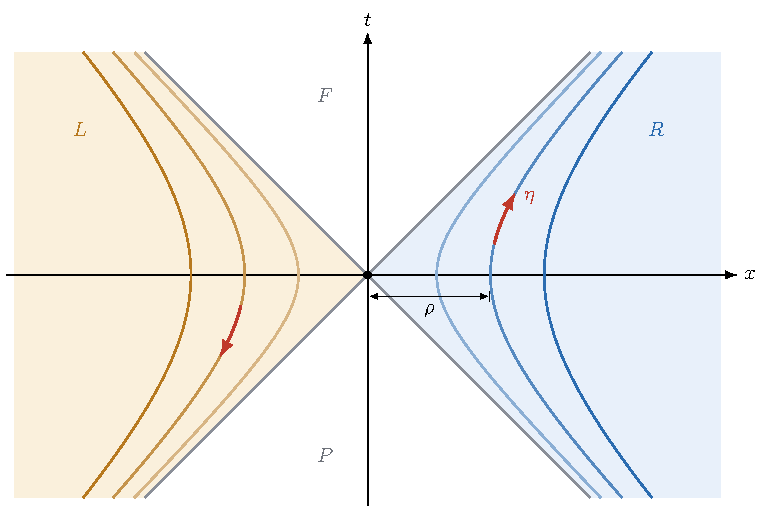
\includegraphics[width=0.82\textwidth]{figs/fig_rindler.pdf}
\caption{The spacetime geometry of the Rindler wedge: Minkowski spacetime split into the Right wedge $R$ ($x > |t|$), Left wedge $L$ ($x < -|t|$), Future $F$, and Past $P$. The boost hyperbolae $x^2 - t^2 = \rho^2$ represent trajectories of uniformly accelerated observers with proper acceleration $a = 1/\rho$, whose proper time $\tau = \rho \eta$ is governed by the boost parameter $\eta$.}
\label{fig:rindler}
\end{figure}

The \textbf{Reeh--Schlieder theorem} — stated here as a fact, with the intuition given, and used repeatedly
from here to the end of the paper — says: in a relativistic quantum field theory, acting on the vacuum
$\ket\Omega$ with operators localized in \emph{any} open spacetime region (however small) produces a set of
states that is dense in the entire Hilbert space. Applied here, this guarantees $\ket\Omega$ is cyclic with
respect to both $\M_R$ and $\M_L$, and hence — by the cyclic-separating duality established in Sec.~IV.A —
cyclic \emph{and} separating with respect to $\M_R$ alone. So Tomita--Takesaki theory applies directly, with
no further assumption needed.

Here is the genuinely striking physical fact, arrived at by using remark (d) from Sec.~IV.A above (find
\emph{any} generator satisfying the KMS condition, and it must be \emph{the} modular operator, since
uniqueness is guaranteed): the modular operator for $\M_R$ in the vacuum state turns out to be
\[
K_\Omega \equiv -\log\Delta_\Omega = 2\pi K
\]
(eq.~4.44), where $K$ is the ordinary \textbf{boost generator} — the same operator that generates Lorentz
boosts in special relativity, an honest geometric symmetry of Minkowski space, with absolutely nothing
abstract or algebraic about its definition. Justifying eq.~4.44 requires checking two things, both genuinely
checkable rather than mysterious: (i) flows generated by $K$ are automorphisms of $\M_R$ — immediate, since a
boost maps the Rindler wedge $\widehat R$ to itself (it's a symmetry of the wedge, by the wedge's very
definition as the region left invariant, as a set, by boosts); and (ii) correlators of boosted operators,
$\braket{\Omega|e^{iK\eta}A(x)e^{-iK\eta}B(y)|\Omega}$ for $x,y\in\widehat R$, satisfy the KMS relation with
$\beta=2\pi$ with respect to the boost parameter $\eta$ (eq.~4.45) — a genuine field-theory computation (not
reproduced here) confirming the KMS property directly on physical correlators.

The physical translation of condition (ii) is exactly the \textbf{Unruh effect}, and it's worth spelling out
the geometry carefully, because ``a Rindler observer'' is not just a figure of speech. Writing the Minkowski
metric as $ds^2=-dt^2+dx^2=-\rho^2d\eta^2+d\rho^2$ (Rindler coordinates: $\rho$ is a radial-like coordinate,
$\eta$ a boost-angle-like coordinate), a trajectory of constant $\rho$ traces out a hyperbola in the $(t,x)$
plane — this is exactly the worldline of an observer undergoing constant proper acceleration $a=1/\rho$, and
$\eta$, the boost parameter, is proportional to that observer's own proper time, $d\tau=\rho\,d\eta$.
Condition (ii) says: observers using $\eta$ as their clock — i.e., \emph{exactly these uniformly accelerated
observers} — experience the ordinary Minkowski vacuum, which contains no particles at all as far as an
inertial observer is concerned, as a genuinely thermal bath, at temperature
\[
T_\rho = \frac{1}{2\pi\rho} = \frac{a}{2\pi} .
\]
This is Unruh's 1976 result, arrived at here as a direct, unavoidable consequence of Tomita--Takesaki theory
applied to the vacuum of a relativistic field, with the specific factor of $2\pi$ in eq.~4.44 being exactly
what converts the universal, dimensionless modular temperature $\beta=1$ into this specific, physical
temperature once $\eta$ is converted to the accelerated observer's own proper time $\tau$.

\begin{figure}[htbp]
\centering
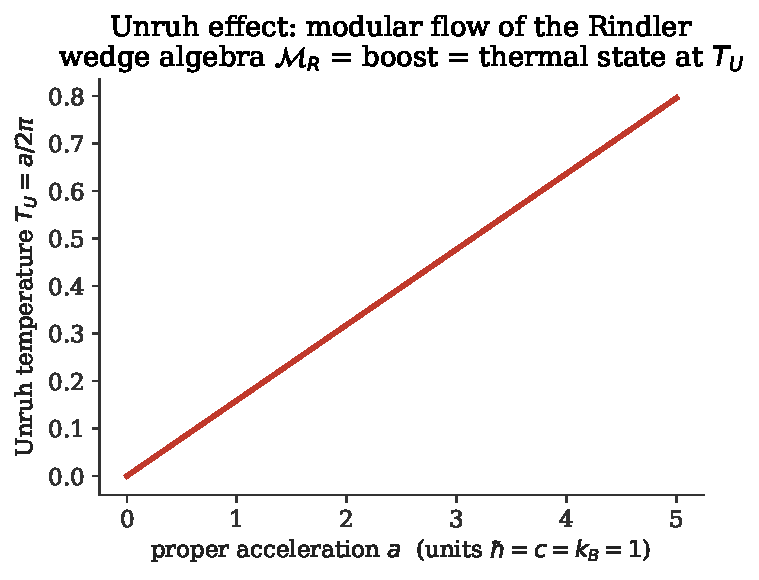
\includegraphics[width=0.78\textwidth]{figs/fig_unruh.pdf}
\caption{The Bisognano--Wichmann theorem and the Unruh effect: the modular flow $\sigma_t^\Omega(A) = \Delta_\Omega^{it} A \Delta_\Omega^{-it}$ acting on the right Rindler wedge $\M_R$ is geometrically equivalent to a Lorentz boost with parameter $\eta = 2\pi t$. Accelerated observers perceive the Minkowski vacuum as a thermal KMS state with local Unruh temperature $T(x) = \hbar c / (2\pi k_B x)$.}
\label{fig:unruh}
\end{figure}

The boost generator $K$ has purely continuous spectrum, all of $(-\infty,\infty)$ (it's the generator of an
honest noncompact symmetry — there's no smallest nonzero boost, and boosts of arbitrarily large rapidity all
exist), so $\Delta_\Omega=e^{-2\pi K}$ has spectrum all of $\mathbb R_{\ge0}$ — and it can be shown that
$S(\M_R)$ coincides with this spectrum, giving (by the classification of Sec.~IV.B) \textbf{$\M_R$ is type
$\mathrm{III}_1$}. The modular conjugation $J_\Omega$ turns out to be exactly $CRT$ — charge conjugation,
combined with a spatial reflection and time reversal — meaning Tomita--Takesaki theory, applied to a
relativistic vacuum, reconstructs the celebrated CPT theorem directly out of nothing but the algebra and the
vacuum state, with no separate argument needed.

This entire story generalizes immediately to higher spacetime dimensions (any transverse directions just ride
along unaffected, since the boost only acts in the $t$-$x$ plane), and — this is the deeper point, worth
holding onto — it generalizes to a \emph{general} open region $O$ on a Cauchy slice, not just the special case
of a half-space. Reeh--Schlieder guarantees $\ket\Omega$ is still cyclic and separating for $\M_O$, so
Tomita--Takesaki theory applies; the modular operator can no longer, in general, be written down in closed
form (it depends on the precise theory and the precise shape of $O$), but a scale-invariance argument (valid
whenever the theory has a scale-invariant UV fixed point — true of essentially any interacting quantum field
theory taken to short enough distances) still pins down its type. The argument: right near the boundary
$\Sigma_O$ of the region $O$, that boundary looks, at short enough distances, just like a flat plane — locally
indistinguishable from the Rindler-wedge geometry just worked out — so
\[
-\log\Delta_\Omega \approx 2\pi K, \qquad \text{very close to } \Sigma_O ,
\]
(eq.~4.46) with $K$ now the boost that locally leaves $\Sigma_O$ fixed, forcing the same continuous spectrum
$\mathbb R_{\ge0}$ and hence, again, type $\mathrm{III}_1$. \textbf{The type $\mathrm{III}_1$ nature of every
local algebra in a relativistic quantum field theory can be traced directly to this local Rindler structure
near any entangling surface, which in turn is a direct consequence of relativistic causal structure itself} —
this is the precise sense in which ``the causal structure of a relativistic QFT requires type
$\mathrm{III}_1$,'' and correspondingly, a \emph{non}-relativistic field theory (with no light-cone structure
forcing this local Rindler behavior near any cut) need not have type $\mathrm{III}_1$ local algebras at all.

\subsubsection*{Sec.~IV.D.2: the split property}

The heuristic picture from Sec.~I — that non-factorization and type III structure come from infinite
entanglement concentrated among short-distance degrees of freedom right at the boundary of a region — can be
made completely precise, and it's worth seeing the precise version, because it resolves what might otherwise
look like a contradiction: how can two regions be infinitely entangled (type III, no factorization) and yet,
intuitively, ``mostly independent'' once you're not sitting exactly on the shared boundary?

Separate $R$ and $L$ by a small but nonzero buffer distance $\epsilon_b$ (so there's a thin strip $I_\epsilon$
of ``no man's land'' between them). The \textbf{split property} states that there \emph{is} a genuine tensor
factorization $\HH=\HH_1\otimes\HH_2$, with
\[
\M_R \subset B(\HH_1)\otimes\id_{\HH_2} \subset \M_L' = \M_{R_\epsilon}, \qquad
\M_L \subset \id_{\HH_1}\otimes B(\HH_2) \subset \M_R' = \M_{L_\epsilon}
\]
(eq.~4.47, where $R_\epsilon\equiv R\cup I_\epsilon$, similarly $L_\epsilon$) — a genuine type I factor,
$B(\HH_1)\otimes\id_{\HH_2}$, sandwiched in between the two type $\mathrm{III}_1$ algebras $\M_R$ and
$\M_{R_\epsilon}$. This says something with real physical bite: once $R$ and $L$ are separated by \emph{any}
nonzero distance, however small, they \emph{can} be completely disentangled — there exist genuine, honest
product states with respect to the factors $\HH_1,\HH_2$, on which $\M_R$ and $\M_L$ act purely separately.
The entanglement obstruction from Sec.~I, in other words, is a purely short-distance, boundary-localized
phenomenon; it evaporates completely the instant you step back even an infinitesimal amount from the shared
edge. More generally, for any two regions $O_1\subset O_2$ whose boundaries don't actually touch (the closure
of $O_1$ sits strictly inside the interior of $O_2$), the split property guarantees a genuine type I factor
$\N$ with $\M_{O_1}\subset\N\subset\M_{O_2}$ (eq.~4.48) — a type I ``buffer'' can always be inserted, as long
as there's any geometric gap at all to insert it into.

The split property is not an extra assumption pulled from nowhere; it can be shown to follow from a technical
condition called the \emph{nuclear property} — a statement about how quickly the theory's energy density
grows at high energies — believed to hold for any ``reasonable'' relativistic QFT. Given the split property,
it can further be shown that $\M_O$, for an open region $O$, is not just type $\mathrm{III}_1$ but also
\textbf{hyperfinite}: it can be built as the weak closure of an increasing sequence of ordinary,
finite-dimensional matrix algebras (exactly the kind of construction used throughout this companion — bigger
and bigger, but always finite, matrices, taken to a limit). A deep uniqueness theorem then applies: hyperfinite
type $\mathrm{III}_1$ von Neumann algebras are, up to isomorphism, all the \emph{same} algebra. The striking
consequence: \textbf{the local algebra of any region in any ``reasonable'' relativistic QFT — free or
interacting, weakly or strongly coupled, any spacetime dimension — is abstractly isomorphic to the local
algebra of any other region in any other such theory.} Different theories are distinguished not by what their
local algebras \emph{are} (abstractly, they're all the same object), but by how those algebras sit relative to
one another — which operators are shared between overlapping regions, how correlators between distant regions
behave, and so on. This is a genuinely surprising, almost counter-intuitive statement, and it's stated here
exactly as strongly as the paper states it, because it's one of the cleanest illustrations of how much
structure the type classification alone captures, and how much it deliberately does \emph{not} capture (the
dynamics, which lives entirely in the relations between algebras, not in any single algebra's abstract type).

Two further, related consequences are worth walking through, because the first comes with an actual proof
sketch worth seeing, and the second is one of the more startling facts in the whole paper.

\textbf{Strong local preparability.} Take the setup of Fig.~5 (regions $R,L$ split by a buffer $I_\epsilon$).
For a general state $\omega$, there's generally a genuine correlation between $R$ and $L$-operators,
$\omega(AB)\ne\omega(A)\omega(B)$ for $A\in\M_R,B\in\M_L$ (eq.~4.49) — nothing surprising there. The startling
claim: using an operation $W$ supported only in the slightly enlarged region $R_\epsilon$ (not $R$ itself, but
$R$ plus the thin buffer strip), it is possible to build a \emph{new} state $\omega_W$ that (i) has
\emph{zero} correlation between $\M_R$ and $\M_L$ at all, and (ii) matches some arbitrarily chosen target
state $\phi$ exactly on $\M_R$, while leaving the state on $\M_L$ completely unchanged from the original
$\omega$ (eqs.~4.50--4.51). This sounds like it should be nearly impossible — locally erase all correlation
with a distant system while simultaneously re-preparing your own region into any state you like, without
touching the distant system at all — and yet it follows in a few lines from the split property and the type
III structure. Here is the argument, worth seeing because it's short: by the split property, $\M_R\subset
B(\HH_1)$, so there's a vector $\ket\xi\in\HH_1$ representing the target state, $\phi(A)=\braket{\xi|A|\xi}$
(justified more carefully in Sec.~IV.G below). The projection $P_\xi=\ket\xi\rangle\langle\xi|\otimes
\id_{\HH_2}$ lies in $\M_{R_\epsilon}$; since $\M_{R_\epsilon}$ is type III, \emph{every} nonzero projection in
it is equivalent to the identity (Sec.~II.B.5's finiteness discussion, pushed to its extreme: in type III,
nothing is finite, so everything is as ``big'' as the whole algebra) — so there's an isometry $W\in
\M_{R_\epsilon}$ with $WW^\dagger=P_\xi$, $W^\dagger W=\id$. Because $W\in\M_{R_\epsilon}\subset\M_L'$, it
commutes with everything in $\M_L$, so $\omega_W(B)\equiv\omega(W^\dagger BW)=\omega(B)$ for $B\in\M_L$
(eq.~4.51) — the $L$-side is untouched, exactly as claimed. And a short algebraic manipulation using
$P_\xi AP_\xi=\phi(A)P_\xi$ (immediate from $\ket\xi$ representing $\phi$) gives $W^\dagger AW=\phi(A)\id$
(eq.~4.52), from which $\omega(W^\dagger ABW)=\phi(A)\omega(B)$ follows directly (eq.~4.53) — exactly the
claimed factorized, re-prepared state.

\textbf{The Connes--St\o rmer transitivity theorem.} For a type $\mathrm{III}_1$ factor, \emph{any} two states
$\phi,\omega$ can be connected to arbitrary precision $\epsilon>0$ by a unitary $W$ \emph{living inside the
algebra itself}, $\|\phi-\omega_W\|<\epsilon$ (eq.~4.54). In words: every state can be prepared, locally, to
arbitrary accuracy, starting from any other state — a statement of ergodicity so strong it's fair to call the
resulting state space \emph{homogeneous}: no state is structurally special or hard to reach from any other,
in sharp contrast to a type I algebra with a nontrivial center, where different superselection sectors are, by
definition, mutually unreachable by anything in the algebra.

\subsubsection*{Sec.~IV.D.3: the collection of algebras $\{\M(O)\}$, and Haag duality}

One closing structural point, worth having on hand because it resurfaces directly in Sec.~VII: the full
collection of local algebras $\{\M(O)\}$, one for every open spacetime region $O$, is expected to satisfy
several basic consistency relations, each one a direct algebraic translation of an ordinary physical
principle. \textbf{Isotony}, $\M(O_1)\subseteq\M(O_2)$ for $O_1\subseteq O_2$ (eq.~4.55): a bigger region
gives access to at least as many operations as a smaller one it contains — this is almost definitional.
\textbf{The time-slice axiom}, $\M(O)=\M(\widehat O)$ (eq.~4.56): because the equations of motion are causal,
operators anywhere in the domain of dependence $\widehat O$ can be re-expressed, via time evolution, in terms
of operators in $O$ itself — so knowing the algebra on a single Cauchy slice already determines it everywhere.
\textbf{Locality (commutativity)}, $\M(O')\subseteq\M(O)'$ (eq.~4.57): operators in the causal complement
$O'$ (spacelike separated from all of $O$) commute with everything in $\M(O)$ — the operator-algebra statement
of ordinary microcausality. When this last relation holds with \emph{equality}, $\M(O')=\M(O)'$, it's called
\textbf{Haag duality} (eq.~4.58) — a strictly stronger statement, saying that literally \emph{every} operator
commuting with $\M(O)$ is already accounted for by the causal complement, with nothing extra hiding outside
that count. Haag duality is not automatic (it can fail for topologically nontrivial regions), but is expected
to hold quite generally for the vacuum sector of an ordinary relativistic QFT on topologically simple regions.
Two further relations — \textbf{additivity}, $\M(O_1\cup O_2)=\M(O_1)\vee\M(O_2)$ (eq.~4.60: no ``extra,''
genuinely nonlocal operators hide in a union that aren't already built from the pieces), and the resulting
\textbf{intersection property}, $\M(O_1\cap O_2)=\M(O_1)\cap\M(O_2)$ (eq.~4.61, which follows from combining
Haag duality and additivity via a short commutant manipulation, eqs.~4.62--4.63) — round out the full package.
A theory satisfying all of these, for every region (not just topologically trivial ones), is called
``complete.'' These relations are worth having memorized in outline, not for their own sake, but because
Sec.~VII builds subregion-subalgebra duality directly on top of exactly this dictionary, translated to the
boundary theory of AdS/CFT.

\subsection{Sec.~IV.E: emergent times from subalgebras — half-sided modular inclusion}

This subsection introduces a second, genuinely distinct notion of emergent time — one that comes not from a
single algebra's own modular flow, but from the relationship between an algebra and a carefully chosen
subalgebra of it. It is a unique feature of type $\mathrm{III}_1$ algebras specifically, and it is exactly the
mechanism, picked up again in Sec.~VII, that lets a single band of boundary time generate the entire interior
of an emergent black-hole horizon.

\subsubsection*{A new, positive ``Hamiltonian'' $G$}

Let $\M$ be a von Neumann algebra with cyclic-separating vector $\ket\Omega$, modular data $\Delta_\M=
e^{-K_\M}$, $J_\M$, as in Sec.~IV.A. Now suppose $\N\subset\M$ is a genuine subalgebra, and $\ket\Omega$
happens to \emph{also} be cyclic for $\N$ (automatically separating too, since $\N\subset\M$ and $\ket\Omega$
is already separating for the bigger algebra $\M$). $\N$ inherits its own modular data, $\Delta_\N=e^{-K_\N}$,
$J_\N$, with respect to the same $\ket\Omega$.

Here is the first new structural fact, and it's worth seeing the one-line reason it's true: because $\N\subset
\M$, the Tomita operator $S_\M$ (built from $\M$ and $\ket\Omega$) is literally an extension of $S_\N$ (built
from the smaller algebra $\N$ and the same $\ket\Omega$) — $S_\M$ agrees with $S_\N$ everywhere $S_\N$ is
defined, but is also defined on the larger domain $\M\ket\Omega\supseteq\N\ket\Omega$. A general fact about
unbounded operators (extending an operator can only make $X^\dagger X$ bigger, never smaller, in the operator
ordering sense) then gives $\Delta_\N\ge\Delta_\M$ (eq.~4.64), i.e., using $-\log$ (which reverses
inequalities for positive operators), $K_\M\ge K_\N$. Define
\[
G \equiv \frac{1}{2\pi}(K_\M-K_\N) \ \ge 0, \qquad G\ket\Omega=0
\]
(eq.~4.65 — the $2\pi$ is just a convenient normalization chosen for what follows; $G\ket\Omega=0$ follows
because both $K_\M$ and $K_\N$ individually annihilate $\ket\Omega$, eq.~4.9 applied to each). $G$ is a
genuinely positive operator, so it deserves to be called a Hamiltonian, and the flow $e^{iGs}$ it generates is
a legitimate new notion of ``time'' — a second one, distinct from either $\M$'s own modular flow or $\N$'s —
that also happens to leave the reference vector $\ket\Omega$ fixed.

\subsubsection*{The half-sided modular inclusion condition, and what it buys you}

Everything so far works for \emph{any} subalgebra $\N\subset\M$ sharing a cyclic-separating vector. Something
much stronger becomes available if $\N$ satisfies one additional geometric-looking condition, called
\textbf{half-sided modular inclusion}:
\[
\N_t \equiv \Delta_\M^{-it}\N\Delta_\M^{it} \subset \N, \qquad \text{for every } t\le0
\]
(eq.~4.81) — flowing $\N$ by $\M$'s \emph{own} modular flow, for negative modular time, always shrinks $\N$
(or leaves it the same), never grows it. When this holds, a theorem (due to Wiesbrock and, independently,
Borchers, building on earlier work) establishes three remarkable consequences at once, none of them assumed —
all derived purely from eq.~4.81:

\begin{enumerate}
\item $K_\M$ and $K_\N$ satisfy the commutation relations of a genuine \textbf{two-dimensional conformal
(M\"obius) algebra} together with $G$:
\[
[K_\M,K_\N] = -4\pi^2i\,G , \qquad [K_\M,G] = 2\pi i\,G
\]
(eq.~4.82, with a companion relation for the modular conjugations, eq.~4.83) — an entire, recognizable piece
of two-dimensional conformal symmetry, produced out of nothing but one algebraic inclusion condition on two
von Neumann algebras.
\item The flow generated by $G$ moves $\M$ into itself for one whole half of the time axis: $e^{iGs}\M
e^{-iGs}\subset\M$ for $s<0$ (eq.~4.84), and in particular $\N=e^{-iG}\M e^{iG}$ (eq.~4.85) — $\N$ is exactly
the image of $\M$ under one unit of this new, $G$-generated time translation. Running $G$ continuously
produces a whole nested, continuously-parametrized family $\N_t\equiv e^{-iGt}\M e^{iGt}$, with $\N_{t_1}
\subset\N_{t_2}\subset\M$ for $t_1<t_2$ and $\N_\infty=\M$ (eqs.~4.89--4.90) — genuinely new time translation,
distinct from $\M$'s own modular flow, acting purely by relating the algebra to smaller and smaller versions
of itself.
\item \textbf{$\M$ must be type $\mathrm{III}_1$.} Half-sided modular inclusion is not just a convenient
technical condition — its very existence forces the ambient algebra to be the ``most chaotic'' type
identified back in Sec.~IV.B.
\end{enumerate}
(The paper builds several further technical objects along the way to this theorem — unitaries $D(t)=\Delta_\M
^{-it}\Delta_\N^{it}$, $V=J_\M J_\N$, and a chain of nested algebras built by repeatedly conjugating with $V$,
eqs.~4.66--4.80 — used to actually \emph{prove} the theorem and to establish that this half-sided-inclusion
structure, once it exists, is completely unique. These are genuine, careful pieces of functional analysis;
they're flagged here so the notation isn't a surprise if you look at the original, but the three numbered
consequences above are the physical content that matters for everything downstream.)

\subsubsection*{The concrete example: light-cone translations in the Rindler wedge}

Here is the worked example the paper gives, and it's worth working through fully, because it turns the
abstract theorem above into something you can literally picture. Take $\M$ to be the algebra of the right
Rindler wedge $\widehat R$ from Sec.~IV.D.1, and let $\N$ be the algebra of the smaller region $\{x^+>0,\,
x^-<-1\}$ (using light-cone coordinates $x^\pm=x^0\pm x^1$) — a wedge-shaped region nested strictly inside
$\widehat R$, shifted over by one unit along the $x^-$ direction (Fig.~6, left panel). Using $K_\M=2\pi K$
(the boost generator, eq.~4.44) to flow $\N$: because a boost acts on light-cone coordinates by simple
rescaling, $x^\pm\to e^{\mp\eta}x^\pm$, flowing the defining condition $x^->-1$ for time $t$ using
$e^{iK_\M t}=e^{2\pi iKt}$ turns it into $x^->-e^{-2\pi t}$ — so
\[
\N_t \equiv e^{iK_\M t}\N e^{-iK_\M t} = \text{algebra of the region } \{x^+>0,\,x^-<-e^{-2\pi t}\}
\]
(eq.~4.95), and since $e^{-2\pi t}>1$ for $t<0$, this region is genuinely \emph{smaller} than the original
$\N$ (it requires $x^-$ to be even more negative) — exactly $\N_t\subset\N$ for $t<0$, precisely the
half-sided modular inclusion condition, verified directly on an explicit geometric example rather than just
asserted abstractly.

Identifying $G$ explicitly here is a short computation using the ordinary Poincar\'e algebra you already know
from special relativity: writing $P^\pm=\tfrac12(P^0\pm P^1)$ for the light-cone components of the momentum
(energy-momentum) operator, the standard commutation relation between the boost generator and momentum,
$[K,P^\pm]=\pm iP^\pm$ (eq.~4.97 — this is just the ordinary statement that a boost rescales energy and
momentum, exactly the way it rescales light-cone coordinates), combined with the definition of $K_\N$ via a
translation of $K_\M$ by the fixed point $a^\mu=(0,-1)$ of $\N$'s own boost symmetry (eq.~4.96), gives directly
\[
K_\N = K_\M - 2\pi P^+ \qquad \Longrightarrow \qquad G = P^+
\]
(eqs.~4.98--4.99, using the definition $G=\tfrac1{2\pi}(K_\M-K_\N)$ from eq.~4.65). \textbf{So in this example,
the abstract ``positive Hamiltonian'' $G$ is nothing more exotic than the ordinary light-cone momentum
operator $P^+$, and the abstract new ``time flow'' it generates is nothing more exotic than ordinary
translation in the $x^-$ direction.} Every one of the general statements 1--3 above (the conformal algebra,
the half-sided translation structure, the forced type $\mathrm{III}_1$ conclusion) can be checked directly on
this example using nothing but ordinary special-relativistic kinematics — and this is exactly the mechanism
that Sec.~VIII will reuse, essentially verbatim, to show that a single band of \emph{boundary} time in
AdS/CFT can generate the entire interior of an emergent black-hole horizon: the interior turns out to be built
by exactly this kind of half-sided-modular-inclusion light-cone translation, with $G$ playing the role of a
genuine, positive bulk momentum.

(One further variant, quickly: taking $\N$ to instead be the region in Fig.~6's right panel gives a half-sided
inclusion on the \emph{positive} $t$-axis instead, $\N_t\subset\N$ for $t\ge0$ eq.~4.92, with correspondingly
sign-flipped relations eq.~4.93--4.94, and a modular translation generator $G=P^-$ instead of $P^+$ — the
mirror-image construction, translating in $x^+$ instead of $x^-$.)

\subsection{Sec.~IV.F: relative modular flows and relative entropy}

Everything in this subsection is a direct generalization of the material already met in Sec.~I (relative
entropy $S(\rho\|\sigma)$) and Sec.~IV.A (the Tomita operator $S_\Psi$) to a version involving \emph{two}
different reference states $\ket\Psi,\ket\Omega$ at once, both cyclic and separating for the same $\M$. The
goal, worth keeping in view through the machinery: produce a version of relative entropy that survives even
when $\M$ is type III (where, as emphasized since Sec.~III, ordinary entropy $S_\M$ cannot be defined at all).

Define a \textbf{relative Tomita operator} exactly analogously to before, but now mapping between the two
reference vectors:
\[
S_{\Psi\Omega}A\ket\Omega = A^\dagger\ket\Psi\ \ (A\in\M), \qquad
S_{\Psi\Omega}A'\ket\Omega = A'^\dagger\ket\Psi\ \ (A'\in\M')
\]
(eq.~4.100), with polar decomposition $S_{\Psi\Omega}=J_{\Psi\Omega}\Delta_{\Psi\Omega}^{1/2}$ (eq.~4.102)
defining the \textbf{relative modular operator} $\Delta_{\Psi\Omega}\ge0$ and \textbf{relative modular
conjugation} $J_{\Psi\Omega}$, exactly the way the ordinary versions were built in Sec.~IV.A, but now
genuinely mixing the two states. (A short algebraic identity, $S_{\Psi\Omega}S_{\Omega\Psi}=\id$, eq.~4.101,
following directly from the definition, forces a relation $J_{\Psi\Omega}=J_{\Omega\Psi}^\dagger$ and
$J_{\Psi\Omega}\Delta_{\Psi\Omega}J_{\Psi\Omega}=\Delta_{\Omega\Psi}^{-1}$, eqs.~4.103--4.104 — a genuine
consistency check, worked out from the polar-decomposition uniqueness, but not needed for what follows.) There
is a two-state generalization of the KMS relation,
\[
\braket{\Psi|AB|\Psi} = \braket{\Omega|B\,\Delta_{\Psi\Omega}\,A|\Omega}, \qquad A,B\in\M
\]
(eq.~4.105, whose short proof, eq.~4.106, is just unpacking the definition of $S_{\Psi\Omega}$ on both
sides) — this single relation lets you convert correlation functions computed in one state, $\ket\Psi$,
directly into correlation functions computed in the other, $\ket\Omega$, and vice versa: genuinely useful
machinery, used freely later without re-derivation whenever the paper needs to compare correlators across two
different reference states.

The flow generated by $\Delta_{\Psi\Omega}$ can be shown to coincide, on $\M$, with the flow generated by the
ordinary (single-state) $\Delta_\Psi$, and on $\M'$ with the flow generated by $\Delta_\Omega$ (eqs.~4.107--
4.108) — and a further intertwining unitary $u_{\Omega\Psi}(s)\equiv\Delta_{\Omega\Phi}^{-is}\Delta_{\Psi\Phi}
^{is}$ (eq.~4.109, built using a third, auxiliary reference $\ket\Phi$, but shown to not actually depend on
which $\Phi$ was used) gives an \emph{explicit construction} of the inner automorphism relating $\sigma_s^\Psi$
and $\sigma_s^\Omega$ promised back in eq.~4.23 of Sec.~IV.B — closing a loop left open there. (A further
family of identities, eqs.~4.110--4.116, work out consistency relations and alternative expressions for these
intertwiners; they are used as technical machinery later and are not reproduced here.)

\subsubsection*{The payoff: relative entropy for type III, and a genuine positivity proof}

Here, finally, is the object that survives everything: for a type III algebra $\M$, no entropy $S_\M(\Omega)$
can be assigned to a single state $\Omega$ — but a \textbf{relative} entropy between two states can be, using
the relative modular operator just constructed:
\[
S_\M(\Psi\|\Omega) \equiv -\braket{\Psi|\log\Delta_{\Omega\Psi}|\Psi} .
\]
(eq.~4.117.) When $\M$ does have a trace (type I or II, with $\Delta_{\Omega\Psi}=\rho_\Omega\rho_\Psi'^{-1}$
in terms of density operators, eq.~4.118), this reduces exactly to the familiar formula
\[
S_\M(\Psi\|\Omega) = \tr(\rho_\Psi\log\rho_\Psi) - \tr(\rho_\Psi\log\rho_\Omega)
\]
(eq.~4.119, matching eq.~1.8 of Sec.~I of this companion) — but eq.~4.117 itself needs no trace to be
well-defined, and survives, completely intact, into type III.

It's worth seeing the positivity of this relative entropy actually proved, rather than just asserted, since it
is short and genuinely instructive: using the elementary calculus inequality $\log x\le x-1$ (true for every
positive real $x$, with equality only at $x=1$ — a fact you can check by noting $f(x)=x-1-\log x$ has
$f(1)=0$ and $f'(x)=1-1/x$, which is negative for $x<1$ and positive for $x>1$, so $x=1$ is the unique global
minimum of $f$, where $f=0$),
\[
-\braket{\Psi|\log\Delta_{\Omega\Psi}|\Psi} \ \ge\ \braket{\Psi|1-\Delta_{\Omega\Psi}|\Psi}
\ =\ -\braket{\Psi|\Psi} + \braket{\Omega|\Omega} \ =\ 0
\]
(eq.~4.120), where the middle equality uses the two-state KMS relation (eq.~4.105) applied with $A=B=\id$, and
the final equality is just $\braket{\Psi|\Psi}=\braket{\Omega|\Omega}=1$ (both are normalized states). So
$S_\M(\Psi\|\Omega)\ge0$ always — the relative entropy is never negative — proved here using nothing beyond
one calculus inequality and the KMS relation already established. This non-negativity is worth contrasting
directly with Sec.~III's finding that the ordinary (non-relative) entropy $S_\M$, in a type II algebra, could
come out negative: relative entropy is the more robust, better-behaved object precisely because it's always
measuring distinguishability from a fixed, explicit reference, never trying to count states from some absolute
zero that a type II or III algebra simply doesn't have.

\subsection{Sec.~IV.G: a canonical purification — the natural cone}

This closing, more technical subsection answers a question that was quietly used without justification in the
strong-local-preparability proof above (Sec.~IV.D.2): given a state $\omega$ on $\M$, is there a
\emph{canonical} choice of purifying vector $\ket\xi\in\HH$ with $\omega(A)=\braket{\xi|A|\xi}$ — and can it
always be chosen to represent a genuine (not just formal) vector?

In general there can be infinitely many different purifying vectors for the same $\omega$ (a simple type I
example: for $\M=B(\HH_1)\otimes\id_{\HH_2}$, any vector in $\HH_1\otimes\HH_2$ that reduces to the right
density matrix on $\HH_1$ works, pure or mixed, and there's no reason to prefer one over another in general).
But if $\HH$ happens to contain \emph{some} cyclic-separating vector for $\M$ at all (a condition called being
in \textbf{standard form} — satisfied, for instance, whenever $\M=\M_O$ for an open region $O$ in the vacuum
sector of a relativistic QFT, courtesy of Reeh--Schlieder, and satisfied automatically by any GNS
representation built from a faithful state, Sec.~II.D), then a genuinely canonical purifying vector
$\ket{\xi_\omega}$ exists (eq.~4.121).

It's constructed as follows: given a fixed cyclic-separating reference $\ket\Omega$, define the \textbf{natural
cone} $P_\Omega$ as the closure of the set $\{Aj_\Omega(A)\ket\Omega : A\in\M\}$, where $j_\Omega(A)\equiv
J_\Omega AJ_\Omega$ (eq.~4.122; an equivalent description, eq.~4.123, is the closure of
$\{\Delta_\Omega^{1/4}A^\dagger A\ket\Omega : A\in\M\}$). Every normal state $\omega$ on $\M$ then has a
\emph{unique} representative vector inside $P_\Omega$ — this is the canonical purification. (It depends on the
choice of $\Omega$ used to build the cone in the first place; a different reference vector gives, in general,
a different natural cone and hence a different canonical purification of the same $\omega$.)

The paper lists several further technical properties of vectors in the natural cone (eqs.~4.124--4.134) — that
inner products between any two vectors in $P_\Omega$ are automatically real and non-negative (eq.~4.126, the
property actually used in the strong-local-preparability argument above, and the one worth remembering); a
decomposition property for vectors fixed by $J_\Omega$ (eq.~4.127); a distance bound relating the vector-space
distance between two purifications to the more abstract distance between the two states they represent
(eq.~4.128); the fact that any two different cyclic-separating vectors within the same natural cone share
\emph{all} of their modular data — the same $J$, the same cone (eqs.~4.129--4.131); how to handle a
cyclic-separating vector that sits \emph{outside} the natural cone, by relating it back with an explicit
unitary correction (eq.~4.132); and the fact that every automorphism of $\M$ can be implemented by a unitary
chosen to preserve the natural cone (eqs.~4.133--4.134). These are the technical tools that make later,
more advanced arguments in the paper watertight; the property that actually matters for the physical content
of this companion is the existence-and-uniqueness statement itself (eq.~4.121) and the positivity property
(eq.~4.126) — both used explicitly already, above.

\bigskip
\noindent This closes Sec.~IV, and with it, every tool needed to talk about entanglement for \emph{any} type
of von Neumann algebra — I, II, and now III. Section~V picks up exactly where remark (f) of Sec.~IV.A left
off: type III has no trace and hence no entropy of its own, which is a real problem if the goal is ever to
compute something like a black-hole entropy using this machinery. The \textbf{crossed product}, introduced
next, is the construction that fixes this — by literally attaching an auxiliary quantum system (a clock) to a
type III algebra and turning it into a type II algebra, which \emph{does} have a trace.
